\chapter{集合的计数}
\label{chap:combinatorics}

有限集合的大小是元素个数。例如四门课中任取一些课程，每一种选择对应一个子集，
计数就是求这样的子集有多少个。答案看似只需逐个列举，但对象稍多时列举既费力又容易重复或遗漏；
我们需要能从问题结构直接算出数量的规则。另一方面，后文比较候选函数时，函数类往往含有无限多个函数，
直接计数没有意义；不过在固定的几个输入上，许多函数会给出相同的输出，这时可以改数不同的输出模式。

本章先建立有限集合的计数方法，再把同样的思路用于函数在有限输入上的输出模式。
前置内容是第~\ref{chap:sets-functions-and-proofs}章的集合运算、函数（特别是双射）、有限求和与数学归纳法。
区间长度与更一般集合的测量将在下一章介绍，因为可数覆盖的构造还需要数列和级数的收敛知识。

\section{有限集合的计数}
\label{sec:comb-families-counting}

计数前必须确定什么算一个结果。从四个对象中依次取两个，$(1,3)$与$(3,1)$是不同的有序记录；
只保留选中的对象时，它们都表示子集$\{1,3\}$。同一批选择采用不同的记录方式，数量就不同。
本节先用双射比较两个集合的大小，再由加法规则、乘法规则推出排列数与组合数，
用它们计数子集与划分，最后处理类别重叠时的校正，以及由子集累计值恢复单个贡献的反演。
以下令$V=\{1,\ldots,n\}$为有限集合，$n\geq0$；数值例子使用$V_0=\{1,2,3,4\}$。

\subsection{基础计数方法}
\label{sec:comb-decomposition-counting}
\label{sec:comb-finite-counting}
\label{sec:comb-classification-products}

全部计数方法都基于三件事：把要数的集合换成一个更容易数的集合；把它分成互不重叠的几类；
或把每个结果拆成依次进行的几步选择。下面先说明这三条规则，再用它们推出排列和组合的公式。

\subsubsection{加法规则和乘法规则}
\label{sec:comb-classification-counting}

\paragraph{双射与计数}
有限集合$A$的元素个数记为$|A|$。“数出$A$有$n$个元素”的含义，就是把元素依次编号为$1,\ldots,n$，
也就是给出一个双射$\{1,\ldots,n\}\to A$。由此得到最基本的计数原则：
若两个有限集合之间存在双射，则它们的元素个数相同。
理由是双射与编号复合仍是双射：若$g:\{1,\ldots,n\}\to A$是编号、$f:A\to B$是双射，则$f\circ g$就是$B$的编号。
这条原则允许我们把难数的集合换成好数的集合，只要找到两者之间的一一对应。
后面计数子集时，就是先把子集一一对应到零一记录。

\paragraph{加法规则}
一项选择若分为互不重叠的几类，可以分别数出各类，再把数量相加。
用集合表示，若有限集合$A_1,\ldots,A_r$两两不交，则
\[
 \left|\bigcup_{i=1}^r A_i\right|=\sum_{i=1}^r|A_i|.
\]
这称为计数的加法规则。它来自编号的拼接：先给$A_1$的元素编号$1,\ldots,|A_1|$，
再接着给$A_2$的元素编号，依此类推；两两不交保证没有元素被编号两次，
各类的并等于全部结果保证没有元素被遗漏，所以最后的编号恰好到$\sum_i|A_i|$。
例如从两本数学书和三本计算机书中选一本，若这两类没有共同的书，共有$2+3=5$种选择。
若同一本书同时列在两类中，就不能直接相加；重叠情形将在容斥原理中处理。

\paragraph{乘法规则}
\phantomsection
\label{sec:comb-stepwise-counting}
一次结果若由若干个位置上的选择组成，并且各位置的任意选择都可组合成结果，就可以用乘法计数。
对有限集合$A_1,\ldots,A_r$，笛卡尔积中的每个结果是一个有序记录，故
\[
 |A_1\times\cdots\times A_r|=\prod_{i=1}^r|A_i|.
\]
这称为计数的乘法规则。$r=2$时，按第一个位置的取值把$A_1\times A_2$分成$|A_1|$类，
第$a$类是$\{a\}\times A_2$，它与$A_2$之间有双射$(a,b)\mapsto b$，所以每类有$|A_2|$个元素；
加法规则给出总数$|A_1|\cdot|A_2|$。一般的$r$再对位置个数用数学归纳法：
$A_1\times\cdots\times A_{r+1}$与$(A_1\times\cdots\times A_r)\times A_{r+1}$之间有显然的双射。
例如第一位取$a,b$之一，第二位取$1,2,3$之一，
共有$2\times3=6$个结果：$(a,1),(a,2),(a,3),(b,1),(b,2),(b,3)$。
长度为$n$的零一记录是$\{0,1\}^n$中的元素，每位有两个选项，因此共有$2^n$条。

分步选择时，后一步的可选对象常依赖前一步的结果，例如先选组长、再从其余人中选记录员。
这时各步的选项集合不同，但只要第$i$步在每种已有记录后都恰有$n_i$个可选结果，
完整记录数仍是$\prod_i n_i$：按第一步的结果分类，每类内部的完整记录数相同，
加法规则把这些相同的数相加，就得到第一步的选项数乘以每类的数量，再对步数归纳。
关键在于选项\emph{个数}不随前面的选择改变，而选项的具体内容可以改变。

\paragraph{等倍归并}
有时直接数出的记录比真正关心的结果多，而每个结果恰好被记录了相同的次数。
设记录的集合$A$按所表示的结果分成若干类，每类恰有$k$个记录，那么结果的个数是$|A|/k$：
加法规则给出$|A|=k\times(\text{结果个数})$。
这一规则要求每个结果被记录的次数\emph{相同}；若次数不同，就不能统一相除。
后面由排列推出组合、由有名称的划分推出无名称的划分，用的都是这条规则。

\subsubsection{排列数和组合数}
\label{sec:comb-permutation-combination-counts}

从同一组对象中选取若干个对象，可以保留它们的位置，也可以只保留选中了谁。
先按位置计数，再合并只因位置不同而重复的记录，就能联系这两类问题。

\paragraph{排列数}
从$n$个不同对象中取出$k$个，按位置排列且不重复，所得有序$k$元组称为一个排列。
以下$k$是满足$0\leq k\leq n$的整数。第一个位置有$n$种选择，
第二个位置剩$n-1$种，依此类推，第$k$个位置有$n-k+1$种；乘法规则给出
\[
 P(n,k)=\prod_{i=0}^{k-1}(n-i)=n(n-1)\cdots(n-k+1).
\]
$k=0$时取空积$1$，对应唯一的空排列。
例如从四人中选出有区别的组长和记录员，有$P(4,2)=4\cdot3=12$种安排。
交换两人的职位会得到不同结果。

把$n$个对象全部排好时，结果数为$n(n-1)\cdots1$，简记为$n!$，
称为$n$的\term{阶乘}（factorial）；约定$0!=1$。利用这个简写，
\[
 P(n,k)=\frac{n!}{(n-k)!}.
\]
这里的阶乘只是连乘记号，排列数的依据仍是前面的分步选择。

\paragraph{组合数}
若只记录选中的对象，结果就是一个$k$元子集，称为一个组合；$k$元子集的个数记为$\binom nk$，称为组合数，读作“$n$选$k$”。
每个排列都确定一个$k$元子集，即它用到的对象；反过来，同一个$k$元子集中的$k$个对象可以按$P(k,k)=k!$种次序排成排列。
所以全部$P(n,k)$个排列按所对应的子集分成$\binom nk$类，每类恰有$k!$个排列。
等倍归并给出$P(n,k)=\binom nk k!$，于是
\begin{equation}
 \binom nk
 =\frac{P(n,k)}{k!}
 =\frac{n!}{k!(n-k)!},
 \qquad 0\leq k\leq n.
 \label{eq:prelim-binomial-coefficient}
\end{equation}
例如十二个有序二人安排中，每个无序小组都出现两次，所以小组数为
$12/2=6$。
从$V_0$选出的六个二元子集是
\[
 \{1,2\},\ \{1,3\},\ \{1,4\},\ \{2,3\},\ \{2,4\},\ \{3,4\}.
\]
约定$\binom nk=0$用于$k<0$或$k>n$；$\binom n0=\binom nn=1$分别对应空集和整个$V$。

\paragraph{组合数的对称性}
选中一个$k$元子集，就同时确定了它的$n-k$元补集。
取补集给这两类子集建立一一对应，因此
\[
 \binom nk=\binom n{n-k}.
\]
例如从四人中选一人，与指定未选中的三人，是同一批选择的两种记录方法。

\paragraph{组合数的总和}
把全部子集按大小分成$0,1,\ldots,n$元子集这$n+1$个互斥类别。
加法规则把各类数量相加。另一方面，全部子集与长度为$n$的零一记录一一对应
（下一小节的幂集计数将写出这一双射），乘法规则给出它们共有$2^n$个，所以
\[
 \sum_{k=0}^n\binom nk=2^n.
\]
例如$n=4$时，各类数量为$1,4,6,4,1$，总数为$16$。
同一个集合按两种方式计数，所得数量必然相等；这种“双重计数”是证明组合恒等式的常用办法。

\paragraph{组合数的拆分 (Pascal恒等式)}

分类还可以得到组合数之间的关系。固定$V$中的一个元素，把$k$元子集分成包含它和不包含它两类。
不包含时，从其余$n-1$个元素选$k$个；包含时，从其余元素再选$k-1$个。因此
\[
 \binom nk=\binom{n-1}k+\binom{n-1}{k-1},\qquad n\geq1.
\]
这就是Pascal恒等式。令$a_{n,k}=\binom nk$，还可写成递推式
\begin{equation}
 a_{n,k}=a_{n-1,k}+a_{n-1,k-1},\qquad n\geq1,
 \label{eq:comb-binomial-recurrence}
\end{equation}
其中$a_{0,0}=1$，范围外的值取$0$。由此依次得到$(1)$、$(1,1)$、$(1,2,1)$、
$(1,3,3,1)$和$(1,4,6,4,1)$。图~\ref{fig:vol1-add-pascal-recurrence}显示$\binom42=3+3$的两类来源。
\begin{figure}[!htb]
  \centering
  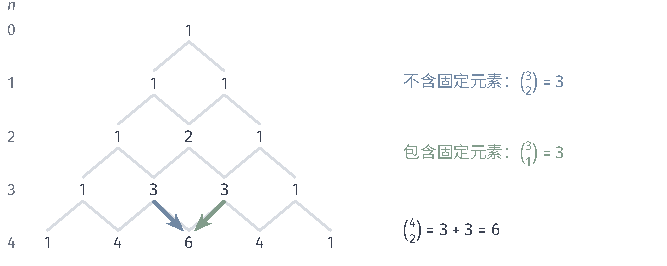
\includegraphics[width=112mm]{figures/01-mathematical-preliminaries-upper/01-mathematical-language-combinatorics-analysis-optimization/tikz/comprehension-additions/pascal-recurrence.pdf}
  \caption{组合数的逐行递推。第$n$行列出$\binom n0,\ldots,\binom nn$；箭头突出$\binom42=\binom32+\binom31=3+3$。两种分类分别从其余三个元素选两个，或先保留固定元素再从其余三个中选一个。网格位置表示递推依赖，不表示子集包含关系。}
  \label{fig:vol1-add-pascal-recurrence}
\end{figure}

\paragraph{组合数的交错和}
交错和$\sum_k(-1)^k\binom nk$把偶数大小子集的个数记为正，奇数大小子集的个数记为负。
当$n\geq1$时，固定$V$中的一个元素$i$，定义映射：若$i\in S$就把$i$删去，若$i\notin S$就把$i$加入。
这个映射作用两次回到原子集，所以是$\mathcal P(V)$到自身的双射；它每次恰好改变子集大小$1$，
因而把偶数大小的子集一一送到奇数大小的子集。两类子集个数相同，正负相抵，因而
\begin{equation}
 \sum_{k=0}^n(-1)^k\binom nk=0,\qquad n\geq1.
 \label{eq:comb-alternating-subset-count}
\end{equation}
$n=0$时只有空集，交错和为$1$。后面的容斥与Möbius反演将用这项抵消关系。

\subsubsection{子集与划分的计数}
\label{sec:comb-subset-partition-counts}

排列和组合数的是固定大小的选择。若不限制选多少个，或者要把全部对象分到几组，
仍可以先用双射换成零一记录，再用乘法规则与等倍归并计数。

\paragraph{幂集}
\phantomsection
\label{sec:comb-ordered-unordered}
若不限制子集大小，结果集合为幂集$\mathcal P(V)$，它包含$V$的所有子集。
每个子集$S$对应一条长度为$n$的零一记录$(z_1,\ldots,z_n)$：第$i$位为$1$表示$i\in S$，为$0$表示$i\notin S$。
不同子集至少在一个元素上不同，记录也就在相应位上不同；任给一条记录，取值为$1$的位置又组成一个子集。
所以这是$\mathcal P(V)$到$\{0,1\}^n$的双射，乘法规则给出
\begin{equation}
 |\mathcal P(V)|=2^n.
 \label{eq:comb-power-set-count}
\end{equation}
例如$V_0$有$16$个子集；$n=0$时，幂集只有空集这一个元素，数量为$2^0=1$。
若只允许其中部分子集，把这些允许的子集组成的集合称为
\term{集合族}（set family），记作$\mathcal F\subseteq\mathcal P(V)$，这与第~\ref{chap:sets-functions-and-proofs}章的集合族是同一概念。
例如只收集$V_0$的二元子集，就得到一个含$\binom42=6$个成员的集合族。

\paragraph{二分划分}
把$V$中的对象分到有名称的两侧，例如“已选”和“未选”，可记为$(S,V\setminus S)$。
结果由第一侧$S$唯一确定，任意$S\subseteq V$也都给出一个结果，所以允许空侧时共有$2^n$个结果。
例如把四门课分别放入“已选”和“未选”两侧，共有$16$种分法。

若两侧没有名称，交换两侧表示同一结果，这时数的是集合$\{S,V\setminus S\}$。
对$n\geq1$，$S$与$V\setminus S$总不相同，因为恰有一个包含元素$1$；
所以每个无名称结果恰有两个有名称表示，等倍归并给出$2^n/2=2^{n-1}$个。
若还要求两侧均非空，就从有名称的结果中去掉$(\varnothing,V)$与$(V,\varnothing)$两个，
有名称和无名称的数量分别为$2^n-2$与$2^{n-1}-1$。例如把四个对象分成两个无名称的非空组，共有$8-1=7$种。
$n=0$时，允许空侧只有$(\varnothing,\varnothing)$一个结果，且两侧相同；要求非空则没有结果。
这时每个无名称结果不再恰有两个表示，等倍归并的条件不成立，不能使用除以$2$的公式。

\subsection{存在重叠关系的计数}
\label{sec:comb-overlap-counting}
\label{sec:comb-inclusion-mobius}

加法规则要求类别不交。若同一元素属于多个集合，直接相加就会重复计算，需要用交集大小校正。

\paragraph{容斥原理}

设$A=\{1,2,3,4\}$、$B=\{3,4,5\}$。$|A|+|B|=4+3=7$把公共元素$3,4$都数了两次，
减去一次交集大小便得到$|A\cup B|=4+3-2=5$。
一般地，把并集分为$A\setminus B$、$A\cap B$与$B\setminus A$三个互斥区域。
加法规则给出$|A|=|A\setminus B|+|A\cap B|$、$|B|=|B\setminus A|+|A\cap B|$，
以及$|A\cup B|=|A\setminus B|+|A\cap B|+|B\setminus A|$。把前两式相加再与第三式比较，可得
\[
 |A\cup B|=|A|+|B|-|A\cap B|.
\]
图~\ref{fig:comb-inclusion-exclusion-overlap}显示需要减掉的正是公共区域多出来的一次计数。
\begin{figure}[htbp]
  \centering
  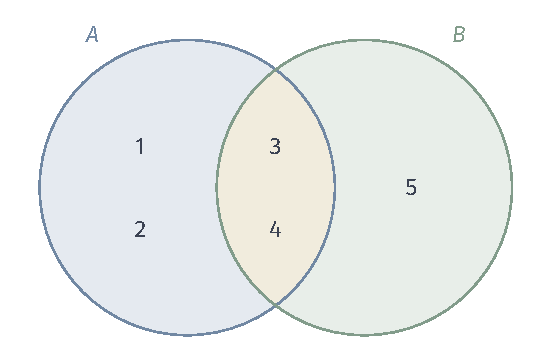
\includegraphics[width=90mm]{figures/01-mathematical-preliminaries-upper/01-mathematical-language-combinatorics-analysis-optimization/tikz/inclusion-exclusion-overlap.pdf}
  \caption{两个有限集合的重叠计数。$A=\{1,2,3,4\}$，$B=\{3,4,5\}$；仅属于$A$的区域放入$1,2$，公共区域放入$3,4$，仅属于$B$的区域放入$5$。把两圈元素个数相加时，公共区域被数两次，减去一次后得到并集中的五个不同元素。}
  \label{fig:comb-inclusion-exclusion-overlap}
\end{figure}

对三个有限集合，逐个元素检查它被计了几次。只属于一个集合的元素在$|A|+|B|+|C|$中计一次，不出现在任何交集中；
恰属于两个集合的元素先计两次，再在一个两两交集中减去一次，最终计一次；
同时属于三者的元素先计三次，在三个两两交集中各减一次后变为$3-3=0$次，
所以还要加回三重交集。因此
\[
 \begin{aligned}
 |A\cup B\cup C|&=|A|+|B|+|C|\\
 &\quad-|A\cap B|-|A\cap C|-|B\cap C|+|A\cap B\cap C|.
 \end{aligned}
\]
在上述例子加入$C=\{4,5,6\}$，两两交集大小为$2,1,2$，三重交集大小为$1$，
并集大小为$4+3+3-2-1-2+1=6$。

\term{容斥原理}（inclusion--exclusion principle）
把这种交替校正推广到任意有限个集合。
\begin{theorem}[有限容斥原理]
\label{thm:comb-inclusion-exclusion}
设$A_1,\ldots,A_m$是有限集合。则
\begin{equation}
  \left|\bigcup_{i=1}^{m}A_i\right|
  =\sum_{\varnothing\neq I\subseteq\{1,\ldots,m\}}
  (-1)^{|I|+1}\left|\bigcap_{i\in I}A_i\right|.
  \label{eq:comb-inclusion-exclusion}
\end{equation}
\end{theorem}

\begin{proof}
沿用三个集合时的思路，逐个元素比较两侧的贡献。左侧中，并集的每个元素恰计一次。
右侧是若干集合大小的带符号和；把每个$|\bigcap_{i\in I}A_i|$写成其中元素各计一次的和，
再按元素合并，就只需检查每个元素$x$在右侧的总系数。
设$x$恰好属于$r$个集合$A_i$，记这些下标组成集合$J$，$|J|=r$。
$x$属于交集$\bigcap_{i\in I}A_i$当且仅当$I\subseteq J$。$r=0$时没有这样的非空$I$，$x$也不在并集中，两侧都不计入它。
$r\geq1$时，大小为$k$的$I\subseteq J$有$\binom rk$个，每个贡献系数$(-1)^{k+1}$，所以$x$在右侧的总系数为
\[
 \sum_{k=1}^r(-1)^{k+1}\binom rk
 =-\left(\sum_{k=0}^r(-1)^k\binom rk-1\right)=1,
\]
最后一步用式~\eqref{eq:comb-alternating-subset-count}：$r\geq1$时交错和为零。
所以并集中的每个元素在右侧也恰好计入一次，两侧相等。
\end{proof}

\paragraph{补集计数}

有些限制条件同时涉及多项要求，直接数满足全部要求的结果比较困难；
不满足要求的结果却可以按“违反哪一条”分别描述。这时先数坏结果，再从总数中减去。
例如四门课的选择用$\bm z=(z_1,z_2,z_3,z_4)\in\{0,1\}^4$表示，$z_i=1$表示选第$i$门课。
要求课程$1,2$恰选一门，选$3$必须选$1$，选$4$必须选$2$或$3$中的至少一门。
违反各条规则的集合分别为
\[
 \begin{aligned}
 A_1&=\{\bm z:z_1=z_2\},\\
 A_2&=\{\bm z:z_3=1,\ z_1=0\},\\
 A_3&=\{\bm z:z_4=1,\ z_2=z_3=0\}.
 \end{aligned}
\]
由De Morgan律，满足全部规则的结果组成$A_1^{\mathrm c}\cap A_2^{\mathrm c}\cap A_3^{\mathrm c}=(A_1\cup A_2\cup A_3)^{\mathrm c}$，
所以合法结果数等于$16-|A_1\cup A_2\cup A_3|$，而后者正好用容斥原理计算。
各项大小都可以用乘法规则读出：$A_1$中$z_1=z_2$的共同取值有$2$种，$z_3,z_4$各有$2$种，故$|A_1|=8$；
$A_2$固定两位、其余两位自由，故$|A_2|=4$；$A_3$固定三位，故$|A_3|=2$。
$A_1\cap A_2$要求$z_1=z_2=0$、$z_3=1$，只剩$z_4$自由，有两个元素；
$A_1\cap A_3$要求$z_2=0$，进而$z_1=0$，又$z_3=0$、$z_4=1$，只有$(0,0,0,1)$；
$A_2\cap A_3$同时要求$z_3=1$与$z_3=0$，为空集，三重交集也就为空。
坏结果共有$8+4+2-2-1-0+0=11$个，
所以合法结果为$16-11=5$个，对应的课程集合族是
\begin{equation}
 \mathcal C_0=\bigl\{\{1\},\{1,3\},\{1,3,4\},\{2\},\{2,4\}\bigr\}.
 \label{eq:comb-running-feasible-family}
\end{equation}
直接核对也得到同样的五个：$z_1=1,z_2=0$时$z_3$可任取，但$z_4=1$要求$z_3=1$，得到三种；
$z_1=0,z_2=1$时必须$z_3=0$，$z_4$可任取，得到两种。

\subsection{Möbius反演}
\label{sec:comb-cumulative-inversion}

容斥原理由各交集的大小恢复并集的大小。类似的问题也出现在更一般的数值上：
设想四门课程组合各有一个“得分”，单门课各有贡献，某两门课同时选又会产生额外的配合效果。
我们能观察到的是每个课程组合的总得分，想知道的却是每个组合自身贡献了多少。
总得分是其全部子组合贡献的累计，恢复单个贡献就是把这种累计倒过来。
本小节先把“给子集赋值”写成集合函数，再给出反演公式并证明它。

\paragraph{集合函数}

以$V$的子集为输入的函数称为集合函数（set function）。例如实值集合函数写作$g:\mathcal P(V)\to\mathbb R$，
元素计数$g(S)=|S|$就是一例。还可以在$W=\{1,3\}$上规定
$g(\varnothing)=0$、$g(\{1\})=g(\{3\})=2$、$g(W)=7$。
这个函数为每个子集给出了实数值，其中二元集合的$7$不等于两个单项值之和，说明集合函数未必可加。
多出来的$7-2-2=3$正是$\{1,3\}$作为一个整体额外贡献的部分；下面的反演公式会把这一计算推广到任意子集。

\paragraph{子集格}

累计沿包含关系进行：$S$的累计值收集所有$T\subseteq S$的贡献。
第~\ref{sec:prelim-binary-relations}节已经说明，包含关系是幂集上的偏序。
有限集合$V$的所有子集按这一偏序排列，组成子集格。它的元素是子集，次序为
$T\subseteq S$；
两个子集的交是它们最大的公共子集，并集是包含两者的最小子集。
例如$\{1\}$与$\{3\}$均包含于$\{1,3\}$，它们的共同下方还有空集。

\paragraph{Möbius反演}

记$h(T)$为子集$T$自身的贡献，$g(S)$为所有$T\subseteq S$贡献的总和。
已知$g$时，可以用下面的\term{Möbius反演}（Möbius inversion）公式恢复$h$。
\begin{theorem}[子集格上的 Möbius 反演]
\label{thm:comb-mobius-inversion}
设$V$为有限集合，$g,h:\mathcal{P}(V)\to\mathbb{R}$满足
\begin{equation}
  g(S)=\sum_{T\subseteq S}h(T)
  \qquad\text{对每个 }S\subseteq V.
  \label{eq:comb-zeta-transform}
\end{equation}
则
\begin{equation}
  h(S)
  =
  \sum_{T\subseteq S}(-1)^{|S|-|T|}g(T).
  \label{eq:comb-mobius-inversion}
\end{equation}
反过来，由式~\eqref{eq:comb-mobius-inversion}定义$h$也会恢复
式~\eqref{eq:comb-zeta-transform}。
\end{theorem}

\begin{proof}
把式~\eqref{eq:comb-zeta-transform}代入反演式右侧。所得双重和遍历满足$R\subseteq T\subseteq S$的全部集合对$(R,T)$，
先固定外层的$T$与先固定$R$遍历的是同一批集合对，所以可以像第~\ref{sec:prelim-finite-sums-products}节的三角形求和那样交换有限求和次序，得到
\begin{align*}
  \sum_{T\subseteq S}(-1)^{|S|-|T|}g(T)
  &=
  \sum_{T\subseteq S}(-1)^{|S|-|T|}
  \sum_{R\subseteq T}h(R)\\
  &=
  \sum_{R\subseteq S}h(R)
  \sum_{T:R\subseteq T\subseteq S}
  (-1)^{|S|-|T|}.
\end{align*}
固定$R$后，满足$R\subseteq T\subseteq S$的集合$T$由$S\setminus R$中哪些元素被加入决定，
即$T=R\cup D$，其中$D\subseteq S\setminus R$可以任意选取，且$|S|-|T|=|S\setminus R|-|D|$。
记$q=|S\setminus R|$，按$|D|=j$分类，大小为$j$的$D$有$\binom qj$个，内层和等于
\[
  \sum_{j=0}^{q}\binom{q}{j}(-1)^{q-j}
  =(-1)^q\sum_{j=0}^q(-1)^j\binom qj
  =\begin{cases}1,&q=0,\\0,&q\geq1,\end{cases}
\]
最后一步用式~\eqref{eq:comb-alternating-subset-count}。
它在$R=S$时为$1$，在$R\neq S$时为$0$，所以全部较小子集的贡献抵消，只留下
$h(S)$。反方向也可直接核对：由反演式定义$h$后，
\[
 \sum_{T\subseteq S}h(T)
 =\sum_{R\subseteq S}g(R)
   \sum_{T:R\subseteq T\subseteq S}(-1)^{|T|-|R|}
 =g(S).
\]
两次内层求和都使用组合数交错和的配对抵消：只有$R=S$时剩一个空集项，其余情形为零。
\end{proof}

\paragraph{反演的算例}

记$\mathbb I\{\text{条件}\}$在条件成立时取$1$，否则取$0$。
下面在$V_0$上取一个教学例子，逐项核对反演公式
\[
 g(S)=2|S|+3\mathbb I\{\{1,3\}\subseteq S\}-\mathbb I\{\{2,4\}\subseteq S\}.
\]
四个单项各贡献$2$，子集$\{1,3\}$另加$3$，子集$\{2,4\}$另加$-1$。
表~\ref{tab:comb-four-element-mobius}列出全部累计值及恢复的贡献。
\begin{table}[htbp]
  \centering
  \begin{tabular}{ccc@{\qquad}ccc}
    \toprule
    $S$ & $g(S)$ & $h(S)$ & $S$ & $g(S)$ & $h(S)$ \\
    \midrule
    $\varnothing$ & $0$ & $0$ & $\{1,2\}$ & $4$ & $0$ \\
    $\{1\}$ & $2$ & $2$ & $\{1,3\}$ & $7$ & $3$ \\
    $\{2\}$ & $2$ & $2$ & $\{1,4\}$ & $4$ & $0$ \\
    $\{3\}$ & $2$ & $2$ & $\{2,3\}$ & $4$ & $0$ \\
    $\{4\}$ & $2$ & $2$ & $\{2,4\}$ & $3$ & $-1$ \\
    $\{3,4\}$ & $4$ & $0$ & $\{1,2,3\}$ & $9$ & $0$ \\
    $\{1,2,4\}$ & $5$ & $0$ & $\{1,3,4\}$ & $9$ & $0$ \\
    $\{2,3,4\}$ & $5$ & $0$ & $V_0$ & $10$ & $0$ \\
    \bottomrule
  \end{tabular}
  \caption{四元素子集格上的累计值与局部贡献。除四个单项、交互
  $\{1,3\}$和$\{2,4\}$外，其余局部贡献均为零。}
  \label{tab:comb-four-element-mobius}
\end{table}

例如$g(\{1,3\})=7$，减去两个单项累计值并加回空集基准，得到
\[
 h(\{1,3\})=7-2-2+0=3.
\]
同样，$h(\{2,4\})=3-2-2+0=-1$。对$S=\{1,2,3\}$，
\[
 h(S)=9-(4+7+4)+6-0=0.
\]
图~\ref{fig:comb-mobius-cumulative-local}比较$\{1,3\}$的四个子集上的累计值与自身贡献。
\begin{figure}[htbp]
  \centering
  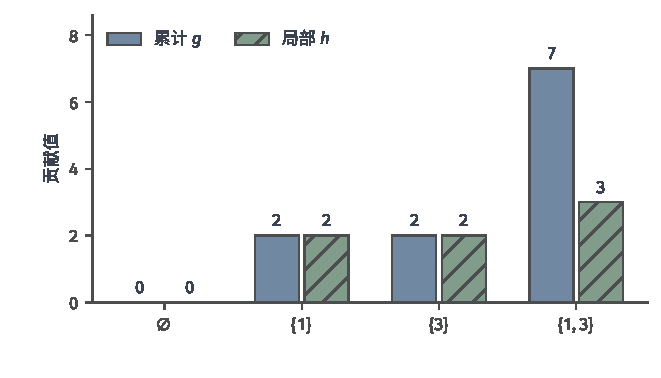
\includegraphics[width=112.0mm]{figures/01-mathematical-preliminaries-upper/01-mathematical-language-combinatorics-analysis-optimization/matplotlib/comb-mobius-cumulative-local/figure.pdf}
  \caption{同一四元素教学构造在$\{1,3\}$的子集上的累计值与局部贡献。左侧蓝柱为$g$，右侧绿斜纹柱为$h$；
 单项贡献各为$2$，二元累计值$7$包含额外交互$3$。图中四个子集的数据由正文解析式精确计算，
 没有省略影响这个二元交互的子集。}
 \label{fig:comb-mobius-cumulative-local}
\end{figure}

反演允许正、负贡献。它与容斥都使用二项式系数的交替抵消，
但容斥保留并集中的每个元素，反演保留指定子集自身的贡献。

\paragraph{Möbius函数}

反演公式中的系数$(-1)^{|S|-|T|}$只依赖两个子集的相对位置。
同样的“由累计值恢复贡献”问题也可以在任意有限偏序集上提出，这时系数由Möbius函数给出。
它由$\mu(S,S)=1$及
\[
 \mu(T,S)=-\sum_{T\preceq R\prec S}\mu(T,R)\qquad(T\prec S)
\]
递归定义，不满足$T\preceq S$时取$0$；这里$\preceq$表示偏序，$\prec$表示偏序且不相等。
递归式的含义是：对每个$S\succ T$，从$T$到$S$之间全部系数之和为零，这正是证明中内层和需要的抵消。
在子集格上，$\mu(T,S)=(-1)^{|S|-|T|}$满足这一递归：对$T\subsetneq S$，记$q=|S\setminus T|\geq1$，
则$\sum_{T\subseteq R\subseteq S}(-1)^{|R|-|T|}=\sum_{j=0}^q(-1)^j\binom qj=0$，
移项正是递归式。所以子集格上的反演系数只取正负一，与定理~\ref{thm:comb-mobius-inversion}一致。

\FloatBarrier
\section{有限输入上的可区分模式}
\label{sec:comb-label-family-capacity}

第~\ref{sec:prelim-function-families}节把候选规则组织成函数族。用观测数据挑选规则时，
我们只看得到每条规则在有限个观测输入上的输出；两条规则若在这些输入上输出相同，数据就无法区分它们。
函数类可以包含无限多个函数，但观察有限个输入时，不同函数给出的输出记录只有有限种，可以用上一节的方法计数。
本节把这些记录称为输出模式，研究两个问题：在给定个数的输入上最多能实现多少种模式；
以及最多能在多少个输入上任意指定输出。前者衡量函数类在有限数据上的区分能力，后者把这种能力概括为一个整数。
二值输出先给出限制类、生长函数和VC维；多分类输出的标签多于两个，改变一个输出有多种选择，需要区分替代标签的要求；
实值输出则先与固定阈值比较，再考虑离阈值的间隔。

\subsection{二值函数类}
\label{sec:comb-vc-growth}

固定非空输入空间$\mathcal X$与非空函数类$\mathcal H\subseteq\{0,1\}^{\mathcal X}$，
这里$\{0,1\}^{\mathcal X}$是第~\ref{sec:prelim-function-definition}节记号下全部$\mathcal X\to\{0,1\}$函数组成的集合。
每个函数在输入处只输出$0$或$1$，例如判断一封邮件是否为垃圾邮件。以下先固定输入，再比较不同输入上的模式数量。

\subsubsection{生长函数}
\label{sec:comb-binary-restrictions}

\paragraph{限制类}

先把观察范围限制在一组固定输入上，只保留函数在这些位置的输出。这样，即使原函数类无限大，当前可以区分的输出记录仍可能只有有限种。

\begin{definition}[限制类]
设$C=\{x_1,\ldots,x_m\}$为互异输入组成的有限集，并固定所列次序。
把每个函数在这些输入上的取值组成一个向量，所有这样的向量构成限制类（restriction）：
\[
 \mathcal H|_C=\{(h(x_1),\ldots,h(x_m)):h\in\mathcal H\}.
\]
\end{definition}
一个向量是一个可实现的输出模式。不同函数若在$C$上取值相同，只在限制类中计一次。
限制类是$\{0,1\}^m$的子集，所以由乘法规则至多有$2^m$个模式，无论$\mathcal H$本身有多大。
例如取$\mathcal X=\mathbb R$，令$\mathcal H=\{h_a:a\in\mathbb R\}$，
其中阈值函数$h_a(x)=\mathbb I\{x\geq a\}$把阈值右侧标为$1$，左侧标为$0$；
这里$\mathbb I\{\text{条件}\}$在条件成立时取$1$，否则取$0$。
在输入$1,2,3$上，模式只取决于阈值$a$落在哪一段：$a\leq1$时为$111$，$1<a\leq2$时为$011$，
$2<a\leq3$时为$001$，$a>3$时为$000$。所以其限制类只有这四个模式，$8$种零一记录中有一半无法实现。
$a=1.5$与$a=1.8$都产生$011$，但在输入$1.7$上取值不同，所以当前模式相同不等于函数相同。

\paragraph{生长函数}

限制类的大小取决于输入位置。固定输入个数后，对所有输入组取最大的模式数，得到生长函数。
\begin{definition}[生长函数]
  \label{def:growth-function}
  生长函数（growth function）记录$m$个输入上最多能区分多少模式。
  对整数\(m\geq0\)，定义
  \begin{equation}
    \Pi_{\mathcal H}(m)
    =\max_{x_1,\ldots,x_m\in\mathcal X}
    |\{(h(x_1),\ldots,h(x_m)):h\in\mathcal H\}|.
    \label{eq:growth-function}
  \end{equation}
  \(m=0\)时只有一个空标记，故\(\Pi_{\mathcal H}(0)=1\)。
\end{definition}

这里允许输入重复，因此有限输入空间也能讨论任意$m$；重复位置必须取得相同标签。
模式数是$1$到$2^m$之间的整数（函数类非空，所以至少有一个模式），有限个整数中总有最大者，
即使输入组有无限多种，可能取到的模式数也只有这些整数，所以定义中的最大值存在。
对阈值函数类，把$m$个互异点从小到大排为$x_1<\cdots<x_m$，模式由阈值落在
$(-\infty,x_1],(x_1,x_2],\ldots,(x_{m-1},x_m],(x_m,\infty)$中哪一段决定，
共$m+1$段，每段给出不同的模式；输入有重复时互异点更少，模式也更少。故$\Pi_{\mathcal H}(m)=m+1$。
例如$m=3$时，恰是前面的四种模式。

\paragraph{指示函数}

二值函数与子集一一对应：函数$h$确定了取值为$1$的输入组成的集合$h^{-1}(\{1\})$，
反过来，给定$S\subseteq\mathcal X$，函数$\mathbb I_S(x)=\mathbb I\{x\in S\}$称为$S$的\term{指示函数}（indicator function）：
它在$S$上取$1$，在$S$外取$0$。因此限制类中的模式也可以看作$C$的子集，即标为$1$的输入组成的集合，
生长函数就可以用有限子集计数求出。
设$\mathcal X$为无限集，固定整数$k\geq0$，令
\[
 \mathcal H_k=\{\mathbb I_S:S\subseteq\mathcal X,\ |S|\leq k\}.
\]
在$m$个互异输入上，正标签位置可以是任意大小不超过$k$的子集，因此
\[
 \Pi_{\mathcal H_k}(m)=\sum_{j=0}^{\min\{k,m\}}\binom mj.
\]
例如$k=1,m=3$时只有$000,100,010,001$，数量为$1+3=4$。
这里统计的是模式数，没有给这些模式规定概率。

\subsubsection{VC维}
\label{sec:comb-binary-shattering-counts}

\paragraph{打散}

若一组输入的全部二值模式都能实现，就可以在这些输入上任意指定标签。
\begin{definition}[打散]
  \label{def:shattering}
  若对有限互异输入集\(C\)的每个二值标记\((b_1,\ldots,b_m)\)，都存在\(h\in\mathcal H\)满足\(h(x_i)=b_i\)对全部\(i\)成立，就称\(\mathcal H\)\term{打散}（shatter）\(C\)。等价地，\(\mathcal H|_C=\{0,1\}^m\)。
\end{definition}

例如阈值函数能在一个点上实现$0$和$1$，所以能打散单点集。
在$x_1<x_2$上却不能实现$10$：若$x_1\geq a$，必有$x_2\geq a$。
因此任意两个点都不能被阈值函数类打散。

\paragraph{VC维}

VC维把能够被打散的输入集大小概括为一个数。
\begin{definition}[VC维]
  \label{def:vc-dimension}
  \(\mathcal H\)的\term{VC维}（Vapnik--Chervonenkis dimension）为
  \[
    \operatorname{VC}(\mathcal H)
    =\sup\{|C|:C\subseteq\mathcal X,\ |C|<\infty,\ C\text{被}\mathcal H\text{打散}\}.
  \]
  空集总能被非空函数类打散，所以维度可为\(0\)；若任意大有限集都能被打散，则取值为\(+\infty\)。
\end{definition}

由刚才的单点与两点判断，阈值函数类的VC维为$1$。
这个数记录可被任意标记的输入数，不是参数个数：
$h_{a,b}(x)=\mathbb I\{x\geq a+b\}$虽写成两个参数，仍是同一个阈值函数类，VC维仍为$1$。

\paragraph{区间指示函数}

此例取$\mathcal X=\mathbb R$、$\mathcal H=\{h_{a,b}:a,b\in\mathbb R,\ a\leq b\}$，
其中$h_{a,b}(x)=\mathbb I\{a\leq x\leq b\}$。
对$x_1<\cdots<x_m$，非空正标签位置只能是连续块$\{i,i+1,\ldots,j\}$。
每个连续块都可由区间选出，再加上全零模式，得到
\[
 \Pi_{\mathcal H}(m)=1+\sum_{i=1}^m(m-i+1)=1+\frac{m(m+1)}2.
\]
两个点的四种模式均可实现；三个点却不能实现$101$，因为包含两端的区间也包含中点。
所以区间函数类的VC维为$2$。图~\ref{fig:comb-interval-shattering-patterns}显示这两项判断。
\begin{figure}[htbp]
  \centering
  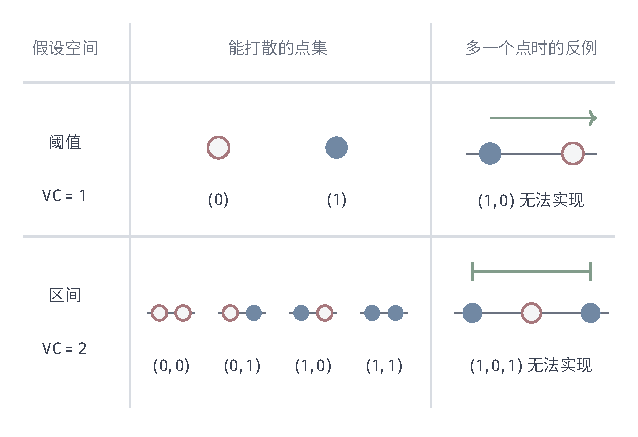
\includegraphics[width=107.999mm]{figures/01-mathematical-preliminaries-upper/01-mathematical-language-combinatorics-analysis-optimization/tikz/comb-interval-shattering-patterns/figure.pdf}
  \caption{阈值与单区间函数类的VC维。中列给出能够打散的输入和相应模式；
 右列给出多一个输入时无法实现的模式。实心点表示标签$1$，空心点表示标签$0$；
 箭头表示阈值的正标签向右延续，线段表示包含两个端点的区间也包含中间点。}
 \label{fig:comb-interval-shattering-patterns}
 \label{fig:learning-vc-shattering}
 \label{fig:learning-vc-dimension-examples}
\end{figure}

图~\ref{fig:combinatorics-growth-patterns}比较区间类的模式数与全部$2^m$个二值模式。
计数相同不要求模式相同：$\mathcal H_2$也有$1+m(m+1)/2$个模式，
但在三个点上缺少$111$，区间类缺少的是$101$。
\begin{figure}[htbp]
  \centering
  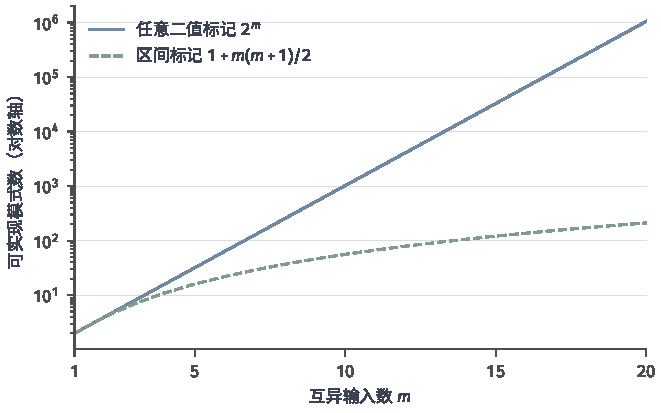
\includegraphics[width=112.0mm]{figures/01-mathematical-preliminaries-upper/01-mathematical-language-combinatorics-analysis-optimization/matplotlib/combinatorics-growth-patterns/figure.pdf}
  \caption{有限输入上的二值模式数（精确计数教学图）。蓝实线为不受限制的\(2^m\)，绿虚线为实数轴区间分类器的\(1+m(m+1)/2\)。纵轴使用对数刻度，绿线是该具体类的精确计数；它也恰等于至多两个正类点的集合族计数，但两类实现的模式可以不同。}
  \label{fig:combinatorics-growth-patterns}
  \label{fig:learning-sauer-growth}
\end{figure}

\FloatBarrier
\Needspace{16\baselineskip}
\paragraph{Sauer--Shelah引理}

阈值类和区间类的模式数都只随$m$多项式增长，远小于$2^m$；它们的VC维也都有限。
这不是巧合：只要VC维有限，生长函数就被一个关于$m$的多项式控制。
为了证明这一点，我们把问题从函数类移到有限的模式族上。
固定输入$x_1,\ldots,x_m$后，限制类是一个模式族$\mathcal A\subseteq\{0,1\}^m$。
称$\mathcal A$打散坐标集$I\subseteq\{1,\ldots,m\}$，是指$\mathcal A$中的模式在$I$的坐标上能实现全部$2^{|I|}$种取值；
$\mathcal H$打散输入$\{x_i:i\in I\}$，恰好意味着限制类打散坐标集$I$。
下面的界由删除最后一个坐标后的分类得到。
\begin{lemma}[Sauer--Shelah引理]
  \label{lem:sauer-shelah}
  若\(d=\operatorname{VC}(\mathcal H)<\infty\)，则对任意\(m\geq0\)，
  \[
    \Pi_{\mathcal H}(m)\leq\sum_{j=0}^{\min\{d,m\}}\binom mj.
  \]
  特别地，当\(1\leq d\leq m\)时，
  \begin{equation}
    \Pi_{\mathcal H}(m)\leq\sum_{j=0}^{d}\binom mj
    \leq\left(\frac{em}{d}\right)^d.
    \label{eq:sauer-shelah}
  \end{equation}
\end{lemma}

\begin{proof}
记$\Phi(m,d)=\sum_{j=0}^{\min\{d,m\}}\binom mj$。我们证明更一般的命题：
任何不能打散超过$d$个坐标的模式族$\mathcal A\subseteq\{0,1\}^m$都满足$|\mathcal A|\leq\Phi(m,d)$。
对$\mathcal H$的任一输入组，限制类不能打散超过$d$个坐标（否则相应输入被$\mathcal H$打散，与VC维为$d$矛盾），
所以这个命题给出引理的第一项结论。

先处理边界情形。$m=0$时只有空模式，$|\mathcal A|\leq1=\Phi(0,d)$。
$d=0$时$\mathcal A$不能打散任何单个坐标；若$\mathcal A$含有两个不同模式，它们在某一坐标上分别取$0$和$1$，
就打散了这个坐标，所以$|\mathcal A|\leq1=\Phi(m,0)$。

对$m,d\geq1$，假定命题对$m-1$个坐标、任意维数上界都成立。
把每个模式删去末坐标，所得前缀组成$U\subseteq\{0,1\}^{m-1}$；
令$W\subseteq U$为既能接$0$又能接$1$的前缀，即$u0$与$u1$都属于$\mathcal A$的前缀$u$。
按前缀给$\mathcal A$的模式分类：每个前缀$u\in U$对应一个或两个模式，恰在$u\in W$时对应两个。
加法规则给出$|\mathcal A|=|U|+|W|$。

$U$不能打散超过$d$个坐标：若$U$打散坐标集$I$，则$\mathcal A$中的模式在$I$上也实现全部取值，故$|I|\leq d$。
$W$不能打散$d$个坐标：若$W$打散某个$|I|=d$的坐标集，则对$I$上的任意取值，都有$W$中的前缀实现它，
而该前缀接$0$或接$1$都在$\mathcal A$中，于是$\mathcal A$打散$I\cup\{m\}$这$d+1$个坐标，产生矛盾。
所以$W$不能打散超过$d-1$个坐标。对$U$与$W$分别使用归纳假设，再用Pascal恒等式逐项合并，便得到
\[
  |\mathcal A|
  \leq\sum_{j=0}^{d}\binom{m-1}{j}
       +\sum_{j=0}^{d-1}\binom{m-1}{j}
  =\binom{m-1}0+\sum_{j=1}^{d}\left[\binom{m-1}j+\binom{m-1}{j-1}\right]
  =\sum_{j=0}^{d}\binom mj,
\]
其中超过坐标数的组合数约定为零，因此这也等于$\Phi(m,d)$。重复输入只会减少可独立取值的坐标，不会增大模式数，
因此对全部输入组取最大值得到第一项结论。

简化界另用初等指数不等式$1+u\leq e^u$（$u\geq0$），其中$e$为自然指数的底；
这一不等式将在第~\ref{chap:function-limits}章由指数函数的级数构造直接读出。
它把有限二项式和写成便于比较的上界，前面的二项式和结论不依赖这一步。
还要比较$\sum_j\binom mja^j$与$(1+a)^m$：把$m$个因子$(1+a)$的乘积逐项展开，
每一项从每个因子中选$1$或$a$；按选出$a$的因子组成的集合分类，选出$j$个$a$的方式恰有$\binom mj$种，每种贡献$a^j$。
因此$\sum_{j=0}^m\binom mja^j=(1+a)^m$，舍去$j>d$的非负项便得下式中的第二个不等号。
当\(1\leq d\leq m\)时，令\(a=d/m\in(0,1]\)。对\(j\leq d\)有\(a^d\leq a^j\)，故
\[
  a^d\sum_{j=0}^{d}\binom mj
  \leq\sum_{j=0}^{d}\binom mj a^j
  \leq(1+a)^m\leq e^{am}=e^d.
\]
除以\(a^d=(d/m)^d\)便得到简化界。\(d=0\)时第一项界为\(1\)，不使用含\(d\)作分母的简化式。
\end{proof}

例如$d=2$时，上界为$1+m+\binom m2$，区间函数类恰好达到它。
这个引理是计数结论；将它用于抽样误差，还需要概率、可测性等条件，
可参考\BookChapterRef{chap:random-sequences-and-processes}{卷2《数学准备：概率、因果与决策》的“随机序列与随机过程”章}。

\subsection{多分类函数类}
\label{sec:comb-multiclass-dimensions}

固定非空输入集合$X$、非空标签集合$Y$和非空函数类$\mathcal H\subseteq Y^X$。
限制类仍记录有限互异输入上的输出向量。二值情形下，打散要求每个输入都能取“另一个”标签，
而另一个标签是唯一的。标签超过两个时，改变一个标签有多种选择，“任意安排输出”就有不同的严格程度：
可以要求在事先固定的两个标签之间任选，可以要求每个模式都能单独改动任一坐标，
也可以只要求能任意决定每个输入是否等于某个参照标签。
下面依次给出这三种要求及相应维数，它们对替代标签的限制由强到弱，最后比较三者的大小关系。

\subsubsection{Natarajan维}
\label{sec:comb-fixed-label-pairs}

\paragraph{Natarajan打散}

Natarajan打散在每个输入上预先固定两个不同标签，再要求实现全部逐点二选一组合。
设$C=\{x_1,\ldots,x_m\}\subseteq X$。若存在$f,g:C\to Y$，
满足每个$x$上$f(x)\neq g(x)$，且对每个$B\subseteq C$都有$h_B\in\mathcal H$满足
\begin{equation}
 h_B(x)=\begin{cases}f(x),&x\in B,\\g(x),&x\in C\setminus B,\end{cases}
 \label{eq:natarajan-shattering}
\end{equation}
就称$C$被$\mathcal H$ \term{Natarajan打散}（Natarajan shattering）。
例如两个输入分别固定标签对$(a,b)$、$(u,v)$时，需要
$(a,u),(a,v),(b,u),(b,v)$四种模式全部出现。

\paragraph{Natarajan维}

固定标签对以后，可以逐个检查哪些输入集允许全部二选一安排。将这些输入集的大小汇总，就得到函数类在这种要求下的维数。

\begin{definition}[Natarajan维]
\label{def:natarajan-dimension}
$\mathcal H$的Natarajan维（Natarajan dimension）为
\[
 d_N(\mathcal H)=\sup\{|C|:C\subseteq X\text{为被}\mathcal H\text{ Natarajan打散的有限集}\}.
\]
没有非空被打散集合时取$0$，可打散任意大有限集时取$+\infty$。
\end{definition}

二标签时，每点的两种标签就是整个$Y$，所以Natarajan维等于VC维。
下面的三标签例子可以逐项检查定义中的四种选择。
\begin{example}[Natarajan维恰为2的有限函数类]
\label{ex:comb-natarajan-concrete}
令输入空间为三封固定邮件$x_1,x_2,x_3$，函数类只含
图~\ref{fig:natarajan-concrete}中的四个函数。在$x_1$上固定标签对“正常、广告”，
在$x_2$上固定“正常、诈骗”，四个函数实现两对标签的全部四种逐点选择，所以
$d_N\geq2$。第三封邮件在四个函数下都预测为正常，任何包含$x_3$的输入集都不能
在该处实现两个不同标签；输入空间只有三点，因此$d_N\leq2$。两项合起来得到
$d_N=2$。
\end{example}

\begin{figure}[htbp]
  \centering
  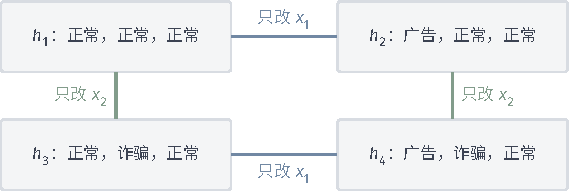
\includegraphics[width=96.28mm]{figures/01-mathematical-preliminaries-upper/01-mathematical-language-combinatorics-analysis-optimization/tikz/natarajan-concrete/figure.pdf}
  \caption{Natarajan打散的四种预测。每个框中的三项依次对应$x_1,x_2,x_3$；
 横向只改变$x_1$，纵向只改变$x_2$，而$x_3$始终预测为正常。
 每个输入处的两个标签预先固定，四个函数实现全部二选一组合。}
 \label{fig:natarajan-concrete}
\end{figure}
\FloatBarrier

\paragraph{生长函数}

当$|Y|=K<\infty$时，沿用式~\eqref{eq:growth-function}对所有输入组取最大值，
定义多分类生长函数$\Pi_{\mathcal H}(m)$，它至多为$K^m$。
有限Natarajan维可将这一上界改进为下面的二项式和。
\begin{theorem}[有限标签的预测数目上界]
\label{thm:multiclass-growth-bound}
设\(2\leq |Y|=K<\infty\)，\(d=d_N(\mathcal H)<\infty\)。
记\(q=\binom K2=K(K-1)/2\)为不同无序标签对的数目，则对每个整数\(m\geq0\)，
\begin{equation}
  \Pi_{\mathcal H}(m)\leq G_{d,K}(m)
  :=\sum_{j=0}^{\min\{d,m\}}\binom mj q^j.
  \label{eq:comb-multiclass-growth-bound}
\end{equation}
\end{theorem}

\begin{proof}
将有限非空模式族\(V\subseteq Y^m\)视为坐标集\(\{1,\ldots,m\}\)上的函数类，
并设其Natarajan维至多为\(d\)。删去末坐标得到前缀族\(U\subseteq Y^{m-1}\)。
对\(u\in U\)，记它能够接上的末尾标签数为\(r(u)\geq1\)。按前缀分类，\(|V|=\sum_{u\in U}r(u)\)，
而\(|U|=\sum_{u\in U}1\)，所以\(|V|-|U|=\sum_u(r(u)-1)\)。
对每个不同标签对\(\{a,b\}\)，令\(U_{a,b}\)为既能接上\(a\)又能接上\(b\)的前缀族。
一个前缀属于\(U_{a,b}\)，当且仅当\(\{a,b\}\)是它能接上的\(r(u)\)个标签中的一对，所以它恰属于\(\binom{r(u)}2\)个\(U_{a,b}\)，
即\(\sum_{\{a,b\}}|U_{a,b}|=\sum_u\binom{r(u)}2\)。又因\(r\geq1\)时\(r-1\leq r(r-1)/2=\binom r2\)，对前缀求和可得
\[
  |V|\leq |U|+\sum_{\substack{\{a,b\}\subseteq Y\\a\neq b}}|U_{a,b}|.
\]
每个无序对在求和中只出现一次。\(U\)的Natarajan维至多为\(d\)。当\(d\geq1\)
时，每个非空\(U_{a,b}\)的Natarajan维至多为\(d-1\)：否则它可以在某\(d\)个
坐标上实现全部固定标签对的选择；每个对应前缀又能接上\(a\)或\(b\)，使\(V\)
在这\(d\)个坐标与末坐标上实现全部二元选择，违反维度上界。空\(U_{a,b}\)的
计数贡献为零。

记\(M(m,d)\)为Natarajan维至多\(d\)的非空模式族\(V\subseteq Y^m\)能够达到的
最大大小，标签集\(Y\)保持固定。对\(m,d\geq1\)，上述分组给出
\[
  M(m,d)\leq M(m-1,d)+qM(m-1,d-1).
\]
零个坐标只有一个空模式，故\(M(0,d)=1\)。维度为零时也至多有一个模式：两个
不同模式必在某坐标上取不同标签，从而Natarajan打散一个坐标。因此\(M(m,0)=1\)。
对\(m\)归纳，将两个较小问题的上界代入，并使用二项式递推关系，得到
\[
\begin{aligned}
  M(m,d)
  &\leq\sum_{j=0}^{d}\binom{m-1}{j}q^j
       +q\sum_{j=0}^{d-1}\binom{m-1}{j}q^j\\
  &=\sum_{j=0}^{d}\binom mj q^j,
\end{aligned}
\]
其中超出坐标数的组合数约定为零。任意输入组上的限制类，其Natarajan维不超过
\(d_N(\mathcal H)\)；重复输入不能作为两个可独立选择的坐标。因此对输入组取最大值，
得到式~\eqref{eq:comb-multiclass-growth-bound}。
\end{proof}

例如$K=3,d=1,m=4$时，$q=3$，界为$1+4\times3=13$，小于全部$3^4=81$种模式。
$K=2$时$q=1$，该公式恢复Sauer--Shelah计数界。

\subsubsection{DS维}
\label{sec:comb-coordinate-replacements}

\paragraph{伪立方体}

另一种要求是不固定标签对，而让每个模式都能单独改变任一坐标，并仍留在同一个有限模式族中。
\begin{definition}[伪立方体]
\label{def:pseudocube}
有限非空集合$V\subseteq Y^m$称为$m$维伪立方体，如果对每个$v\in V$和
每个$i\in\{1,\ldots,m\}$，都存在$u\in V$满足
$u_i\neq v_i$且$u_j=v_j$对所有$j\neq i$成立。
\end{definition}

例如取三个互异标签$a,b,c$，
\[
 \mathcal V=\{(a,a),(a,b),(b,b),(b,c),(c,c),(c,a)\}
\]
是二维伪立方体：每个模式沿第一、第二坐标都能找到一个邻居。
它却不含固定两标签对形成的四个角。图~\ref{fig:comb-multiclass-pattern-grid}把六个模式列入表格，
每行每列都有两个模式，但没有完整的二行二列矩形。
\begin{figure}[htbp]
  \centering
  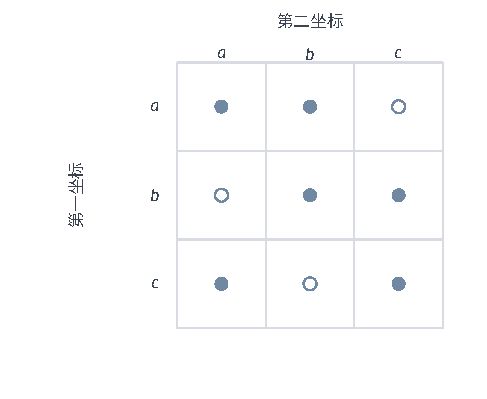
\includegraphics[width=82.501mm]{figures/01-mathematical-preliminaries-upper/01-mathematical-language-combinatorics-analysis-optimization/tikz/comb-multiclass-pattern-grid/figure.pdf}
  \caption{六模式族$\mathcal V$的精确占位图。实心点表示模式属于该族，空心点表示缺失模式。每行每列恰有两个实心点，却没有完整的四角矩形；这不是两个标签的完整立方体。}
 \label{fig:comb-multiclass-pattern-grid}
\end{figure}

\paragraph{DS打散}

若$m$个互异输入组成的有序点集$C$满足$\mathcal H|_C$包含一个$m$维伪立方体，
称$C$被\term{DS打散}（DS shattering）。例如把上述六模式作为两个输入上的全部限制类，
这两个输入便被DS打散，因为六个模式构成二维伪立方体。

\paragraph{DS维}

把能够逐坐标替换的输入规模汇总，就得到Daniely--Shalev-Shwartz维，简称DS维；
下面采用有限伪立方体的表述\scite{brukhim2022multiclass}。
\begin{definition}[DS维]
\label{def:ds-dimension}
DS维$d_{DS}(\mathcal H)$为可被DS打散的有限输入集大小的上确界。
空集给出大小$0$；若任意大的有限集都能被DS打散，维数取$+\infty$。
\end{definition}

对只有两个输入的函数类$\mathcal V$，上述六个模式构成二维伪立方体，因此$d_{DS}=2$。
没有四角矩形意味着不能Natarajan打散两个输入，而一个输入可以取不同标签，故$d_N=1$。
图~\ref{fig:ds-six-cycle}标出每个模式沿两个坐标的邻居。
\begin{figure}[htbp]
  \centering
  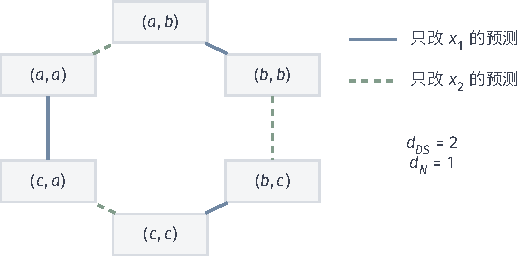
\includegraphics[width=89.02mm]{figures/01-mathematical-preliminaries-upper/01-mathematical-language-combinatorics-analysis-optimization/tikz/ds-six-cycle/figure.pdf}
  \caption{六模式族$\mathcal V$的逐坐标邻接。每个顶点是一种两输入预测；
 蓝实线只改变第一坐标，绿虚线只改变第二坐标。每个顶点在两个方向上都有邻居，
 所以它构成二维伪立方体；图中没有固定两标签对形成的四角矩形，故其
 DS维为2而Natarajan维为1。}
 \label{fig:ds-six-cycle}
\end{figure}

\subsubsection{图维}
\label{sec:comb-reference-labels}

\paragraph{图打散}

图打散先固定每点的参照标签，再要求任意一部分输入匹配参照、其余输入不匹配。
不匹配时采用哪个标签不必预先指定。
\begin{definition}[图打散]
\label{def:graph-dimension}
若有限集$C\subseteq X$存在$f:C\to Y$，使每个$B\subseteq C$都对应某个
$h_B\in\mathcal H$，满足
\[
 h_B(x)=f(x)\ (x\in B),\qquad h_B(x)\neq f(x)\ (x\in C\setminus B),
\]
则称$C$被$\mathcal H$图打散。
\end{definition}

例如参照标签为$(a,u)$时，$(a,u),(a,v),(b,u),(c,w)$分别实现全匹配、只匹配第一处、
只匹配第二处和全不匹配，其中$v\neq u$、$b,c\neq a$、$w\neq u$。

\paragraph{图维}

图打散判断一组输入能否独立安排匹配与不匹配。把能够这样安排的输入数概括为一个上界，就得到对应的维数。

\begin{definition}[图维]
\label{def:graph-dimension-value}
图维（graph dimension）记录可独立安排这种匹配关系的最大点数。
设$\mathcal C_G$为所有被$\mathcal H$图打散的有限输入集组成的集合，定义
\[
 d_G(\mathcal H)=\sup_{C\in\mathcal C_G}|C|.
\]
\end{definition}

\begin{example}[图维恰为2的有限函数类]
\label{ex:comb-graph-shattering-concrete}
令输入空间为$\{x_1,x_2,x_3\}$，函数类只含图~\ref{fig:graph-shattering-concrete}
中的四个函数。以$f(x_1)=a,f(x_2)=u$为基准，四个函数在前两个输入上分别实现
“两处都匹配、只匹配第一处、只匹配第二处、两处都不匹配”，所以
$\{x_1,x_2\}$被图打散。第三个输入始终取$z$，任何包含$x_3$的集合都不能在该处
独立安排匹配与不匹配；输入空间又只有三个点，故这个函数类的图维恰为2。
\end{example}

\begin{figure}[htbp]
  \centering
  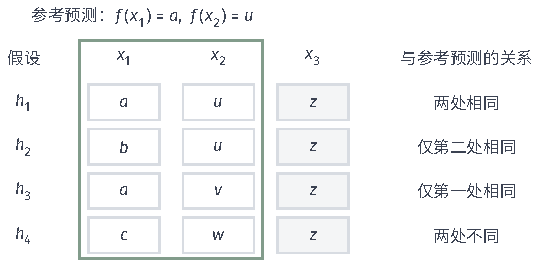
\includegraphics[width=91.401mm]{figures/01-mathematical-preliminaries-upper/01-mathematical-language-combinatorics-analysis-optimization/tikz/graph-shattering-concrete/figure.pdf}
  \caption{图打散与图维的有限例子。框线圈定的两列相对于参考函数实现全部四种匹配或
 不匹配组合；第三列固定为$z$。同一输入偏离基准时可以采用不同标签，
 因而图打散没有预先固定唯一的替代标签。}
 \label{fig:graph-shattering-concrete}
\end{figure}

\paragraph{维数比较}

三种维数分别要求固定标签对、逐坐标邻居和匹配参照标签，按对替代标签的限制由强到弱排列。
表~\ref{tab:comb-multiclass-dimensions}列出条件，图~\ref{fig:learning-multiclass-dimensions}显示对应模式。
\begin{table}[htbp]
  \centering
  \begin{tabular}{p{0.17\linewidth}p{0.70\linewidth}}
    \toprule
    维度 & 在有限输入上的要求\\
    \midrule
    Natarajan维 & 每点固定两个不同标签，全部\(2^m\)种逐点二选一组合均可实现\\
    DS维 & 包含有限非空模式族，每个模式在任一坐标都可单独改变并仍留在族中\\
    图维 & 每点固定一个基准标签，任意点集上匹配、其补集上不匹配的模式均可实现\\
    \bottomrule
  \end{tabular}
  \caption{多类别组合维度的不同量词。图维中的“图”指标记相等关系的图打散，不是输入关系图的顶点数。}
  \label{tab:comb-multiclass-dimensions}
\end{table}

\begin{figure}[htbp]
  \centering
  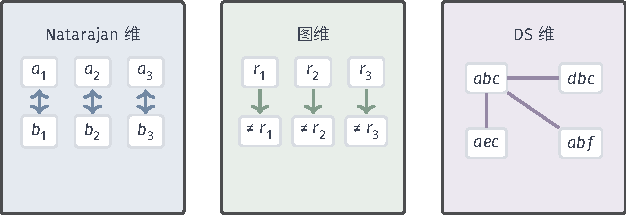
\includegraphics[width=106.056mm]{figures/01-mathematical-preliminaries-upper/01-mathematical-language-combinatorics-analysis-optimization/tikz/learning-multiclass-dimensions/figure.pdf}
  \caption{多分类维度关注的三种结构。Natarajan维固定每个输入处的两个标签，
 图维固定一个基准标签并区分匹配与不匹配，DS维考察预测向量之间只改变一个坐标的
 邻接。右栏只展示局部邻接方式；完整伪立方体还要求每个模式在每个坐标上都有邻居。}
 \label{fig:learning-multiclass-dimensions}
\end{figure}
\FloatBarrier

三种打散要求对替代标签作出的限制不同，但同一组预测模式可以同时接受这些检验。下面比较由这些要求得到的维数，并说明标签数有限时还能推出什么。

\begin{theorem}[多分类维度的比较]
\label{thm:multiclass-dimension-comparison}
对任意非空标签空间与非空函数类，有
\[
  d_N(\mathcal H)\leq d_{DS}(\mathcal H)\leq d_G(\mathcal H).
\]
二标签时三者均等于VC维。若\(|Y|=K<\infty\)，则\(d_N(\mathcal H)<\infty\)
也蕴含\(d_G(\mathcal H)<\infty\)。
\end{theorem}

\begin{proof}
若\(m\)个输入被Natarajan打散，每个坐标的两个候选标签固定，全部\(2^m\)种
选择组成一个有限非空模式族。任意模式都能只翻转任一坐标上的选择并仍留在族中，
所以它是\(m\)维伪立方体，证明\(d_N\leq d_{DS}\)。

若限制类包含\(m\)维伪立方体\(V\)，固定\(v\in V\)作为基准。任取希望偏离基准
的坐标集\(I\subseteq\{1,\ldots,m\}\)，逐个沿\(I\)中的坐标移动到邻居，每个
坐标只移动一次。每一步仅改变当前坐标；之前改变的坐标保持不变，\(I\)之外的
坐标始终与\(v\)相同。因此最终模式恰在\(I\)上不等于\(v\)，在其补集上等于
\(v\)。令\(I\)遍历所有子集就得到图打散，故\(d_{DS}\leq d_G\)。

二标签时，偏离基准的标签唯一。图打散因此要求全部二元模式；伪立方体从任意模式
逐坐标翻转也能到达全部二元模式。Natarajan打散中的两标签正是整个标签集，所以
三种维度都等于VC维。

若\(K=1\)，函数类在任何输入上只有一种标记，三种维度均为零。若\(2\leq K<\infty\)
且\(d_N=d<\infty\)，图打散\(m\)个输入至少需要\(2^m\)个不同模式。由定理~
\ref{thm:multiclass-growth-bound}，必有\(2^m\leq G_{d,K}(m)\)。固定\(d,K\)后，
当$d=0$时，右侧为$1$，所以只能有$m=0$。当$d\geq1$且$m\geq2(d+1)$时，
大小为$d+1$的子集只是全部$2^m$个子集中的一类，再利用组合数的连乘公式，可得
\[
 2^m\geq\binom m{d+1}\geq\frac{(m/2)^{d+1}}{(d+1)!},
 \qquad
 G_{d,K}(m)\leq C m^d,
\]
其中$C=\sum_{j=0}^d q^j/j!$只依赖$d,K$。与$2^m\leq G_{d,K}(m)$合并并约去$m^d$，
得到$m\leq2^{d+1}(d+1)!C$。较小的$m<2(d+1)$也已有有限上界，故图维有限。
\end{proof}

六模式族$\mathcal V$以$(a,a)$为参照时，$(a,a),(a,b),(c,a),(b,b)$实现四种匹配安排，
所以$d_G=2$。该例的三个维数依次为$1,2,2$。
有限标签条件用于计数界。例如无限标签集$Y$上的全部常值函数$h_y(x)=y$，
三个维数都为$1$，但在单个输入上已有无限多个模式，不能套用含有限$K$的计数公式。

\subsection{实值函数类}
\label{sec:comb-real-valued-threshold-margins}

以下固定非空输入空间$\mathcal X$与非空函数类$\mathcal F\subseteq\mathbb R^{\mathcal X}$。
实数输出在单点上就可能无限多；与其计数精确数值，可以先固定每个输入的阈值，
只记录输出在阈值哪一侧。加入正间隔后，还能描述在给定尺度下能否作出这些选择。

\subsubsection{伪维}
\label{sec:comb-threshold-patterns}

\paragraph{伪打散}

实值函数在单个输入上就能取无限多个值，若按精确数值计数，限制类往往无限，前面的计数没有意义。
把实数输出转化为二值信息的最直接办法，是与一个阈值比较，只记录输出在阈值上方还是下方。
对每个输入先选一个阈值，再检查全部高低组合是否可由函数实现，这称为伪打散。
阈值对全部模式保持不变，实现不同模式的函数则可以不同。
\begin{definition}[伪打散]
\label{def:pseudo-shattering}
设$\mathcal F\subseteq\mathbb R^{\mathcal X}$。有限集$C=\{x_1,\ldots,x_m\}$被
$\mathcal F$\term{伪打散}（pseudo-shattering），是指存在$r_1,\ldots,r_m\in\mathbb R$，使任意
$\bm b\in\{0,1\}^m$都对应某个$f_{\bm b}\in\mathcal F$，满足
\[
 b_i=1\Rightarrow f_{\bm b}(x_i)>r_i,\qquad
 b_i=0\Rightarrow f_{\bm b}(x_i)<r_i\quad(1\leq i\leq m).
\]
这里$\Rightarrow$表示“只要左侧条件成立，右侧便须成立”。
\end{definition}

例如取常值函数类$\mathcal F=\{f_a:a\in\mathbb R\}$，其中$f_a(x)=a$。
在一个输入处取阈值$0$，用$a=1$和$a=-1$便能实现高、低两种模式。
两个输入则不能被它伪打散：若阈值$r_1\leq r_2$，要求第一处低于$r_1$、第二处高于$r_2$，
同一个常数不可能同时满足；$r_2\leq r_1$时交换两处即可。

\paragraph{伪维}

常值函数的例子表明，可任意安排高低模式的输入数可能受到限制。伪维用一个数记录这种独立选择能够覆盖的输入规模。

\begin{definition}[伪维]
\label{def:pseudo-dimension}
$\mathcal F$的\term{伪维}（pseudo-dimension）为
$\operatorname{Pdim}(\mathcal F)=\sup\{|C|:C\text{为被}\mathcal F\text{伪打散的有限集}\}$，
允许值为$+\infty$；没有非空被打散集合时值为$0$。
\end{definition}

由刚才的一点、两点判断，常值实函数类的伪维为$1$。
对二值函数类取阈值$1/2$，伪打散就是VC打散，因此伪维与VC维一致。

\subsubsection{胖打散维}
\label{sec:comb-margin-patterns}

\paragraph{胖打散}

\term{胖打散}（fat shattering）要求输出不仅位于阈值两侧，还要与阈值相距至少一个给定正数$\gamma$。
\begin{definition}[胖打散]
\label{def:fat-shattering}
给定$\gamma>0$，若有限集$C=\{x_1,\ldots,x_m\}$存在固定阈值$r_1,\ldots,r_m$，
使任意$\bm b\in\{0,1\}^m$均对应$f_{\bm b}\in\mathcal F$满足
\begin{equation}
 b_i=1\Rightarrow f_{\bm b}(x_i)\geq r_i+\gamma,\qquad
 b_i=0\Rightarrow f_{\bm b}(x_i)\leq r_i-\gamma,
 \label{eq:fat-shattering}
\end{equation}
则称$C$在尺度$\gamma$下被$\mathcal F$胖打散。
等价地，以$\sigma_i=2b_i-1$编码，可写为
\begin{equation}
 \sigma_i\bigl(f_{\bm\sigma}(x_i)-r_i\bigr)\geq\gamma
 \quad(i=1,\ldots,m).
 \label{eq:functional-fat-shattering}
\end{equation}
\end{definition}

例如输入空间只有一个点，函数类在该点的输出只能取$19.999$和$20.001$，固定阈值$20$。
它能实现高、低两种模式，并能留下间隔$\gamma=0.001$，却不能留下间隔$1$。
这说明跨过阈值和以给定幅度跨过阈值是不同要求。

\paragraph{胖打散维}

同一函数类在不同间隔要求下，能够独立安排的输入数可能不同。固定尺度后，再汇总所有满足胖打散要求的输入集大小，就得到相应的维数。

\begin{definition}[胖打散维]
\label{def:fat-shattering-dimension}
尺度$\gamma$下的\term{胖打散维}（fat-shattering dimension）为
$\operatorname{fat}_\gamma(\mathcal F)=
\sup\{|C|:C\text{为在尺度}\gamma\text{下被}\mathcal F\text{胖打散的有限集}\}$。
采用与伪维相同的$0$及$+\infty$约定。
\end{definition}

固定尺度后，胖打散维记录能同时满足该间隔要求的输入数目。
例如上面只有两个常值输出的函数类，在$0<\gamma\leq0.001$时维数为$1$，在$\gamma>0.001$时为$0$。

\paragraph{单调性}

增大$\gamma$只会加强要求，所以$\operatorname{fat}_\gamma(\mathcal F)$关于$\gamma$单调不增。
因$\gamma>0$保证每个见证严格位于阈值一侧，还得到
$\operatorname{fat}_\gamma(\mathcal F)\leq\operatorname{Pdim}(\mathcal F)$。
反过来，一个被伪打散的固定有限集，在某个正尺度下也被胖打散：
从有限种模式各选一个见证函数，取它们在各输入处距阈值的最小距离即可。
这个距离为正，但依赖输入集和所选函数，不能替代预先指定的尺度。

\Needspace{8\baselineskip}
\paragraph{分块常值函数}

下面用可以直接计算的函数类说明幅度限制的作用。
\begin{example}[分块常值函数的胖打散维]
\label{ex:comb-piecewise-constant-fat-dimension}
设非空集合$A_1,\ldots,A_m$构成$\mathcal{X}$的一个划分，并令
\[
  \mathcal{F}_B
  =
  \left\{
    \sum_{j=1}^{m}a_j\mathbb{I}_{A_j}:
    |a_j|\leq B
  \right\},
  \qquad B>0.
\]
当$0<\gamma\leq B$时，从每个$A_j$选一点并取阈值$r_j=0$；对任意符号模式令
$a_j=\gamma\sigma_j$，便能以间隔$\gamma$实现该模式，所以这$m$个点被胖打散。反过来，
任意$m+1$个点中至少两个落在同一个$A_j$内，而类中每个函数在这两个点取值相同。若二者
的阈值为$r$与$r'$且能够被胖打散，模式$(+1,-1)$要求$r'-r\geq2\gamma$，模式
$(-1,+1)$又要求$r-r'\geq2\gamma$，二者矛盾。因此该尺度下的胖打散维恰为$m$。
当$\gamma>B$时，
单点上的两个符号也要求函数值之差至少为$2\gamma$，超过允许区间$[-B,B]$的宽度$2B$，
故胖打散维为$0$。这个算例把分区数控制的自由方向与系数上界控制的可分辨幅度分开了。
\end{example}

图~\ref{fig:comb-fat-margin-output-square}取两个分块、$B=1$，
把两处输出表示为平面中的一个点。四种高低模式能否实现，取决于间隔区域是否仍与允许的正方形相交。
\begin{figure*}[htbp]
  \centering
  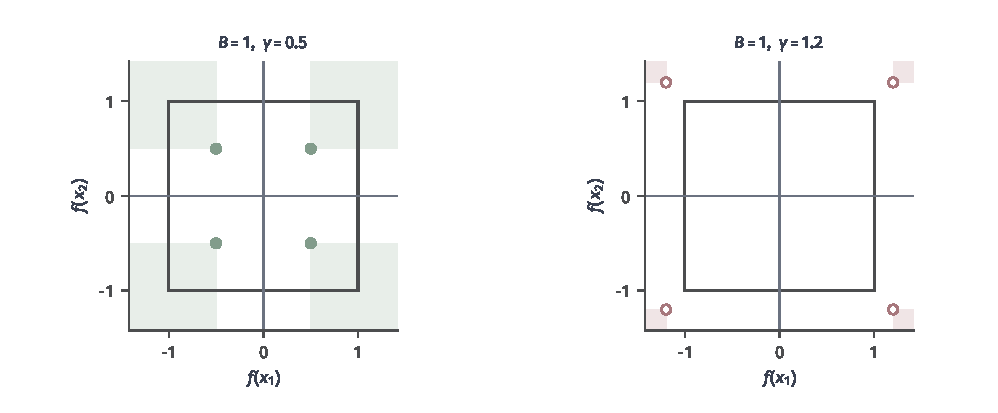
\includegraphics[width=169.0mm]{figures/01-mathematical-preliminaries-upper/01-mathematical-language-combinatorics-analysis-optimization/matplotlib/comb-fat-margin-output-square/figure.pdf}
  \caption{两个分块、$B=1$与固定阈值$r_1=r_2=0$的输出几何。灰框是函数类允许的
 $(f(x_1),f(x_2))\in[-1,1]^2$；浅色区域要求两坐标分别离阈值至少$\gamma$。
 左图的浅绿区域对应$\gamma=0.5$，四种符号可由实心点实现；右图的浅红区域对应$\gamma=1.2$，空心点只标出要求的边界，
 全部落在允许框之外，因而不是类中的函数输出。图为解析教学构造。}
 \label{fig:comb-fat-margin-output-square}
 \label{fig:fat-shattering-example}
\end{figure*}

限制类记录具体模式，生长函数记录模式数，打散维数记录满足相应打散条件的输入规模。
实值函数的伪维与胖打散维分别采用固定阈值和正间隔。
它们与函数空间中的距离、覆盖数是不同概念；后者可参考第~\ref{chap:functional-analysis-and-approximation}章。

\section{本章小结}
\label{sec:comb-summary}

有限计数首先要确定结果的身份：排列保留次序，组合只记录子集，分组还要说明各部分是否有名称。
所有计数都建立在三条规则上：双射把难数的集合换成好数的集合，互斥类别使用加法，完整分步选择使用乘法；
每个结果被重复记录同样多次时，用等倍归并相除。由此得到排列数、组合数、幂集与二分划分的数量，
双重计数与配对又给出组合数的总和、Pascal恒等式和交错和。类别重叠时，容斥用交集校正重复，
补集计数借助De Morgan律把“满足全部限制”改写为“不违反任何一条”。
Möbius反演进一步处理集合的实值累计函数，从累计值恢复各子集的贡献，其系数来自同一种交错抵消。

函数类可能含有无限多个函数，但在有限输入上只有有限种输出模式。限制类记录固定输入上的模式，
生长函数记录最多有多少模式，VC维记录最多能在多少个输入上任意指定二值输出。
Sauer--Shelah引理说明，VC维有限时模式数只随输入数多项式增长，而不是指数增长。
多分类需要明确替代标签的要求，Natarajan维、DS维与图维依次放宽这一要求；
实值函数则通过阈值和间隔形成可比较的模式，得到伪维与胖打散维。

计数始终需要说明什么算一个结果，以及同一个结果会被当前记录方式表示几次。
下一章转向无限过程：先研究数列与函数的趋近，并在级数的基础上把区间长度推广到集合测量，
再建立函数的微分与积分。
